This chapter is directed towards administrators and developers who want to
set up a server and install the software needed to get a fully functional system.
It also contains instructions on how to maintain the system in case problems arise.

\section{A brief introduction to
vagrant}\label{sec:a-brief-introduction-to-vagrant}

\subsection{Basic usage}\label{sec:basic-usage}

Vagrant is configured by a \texttt{Vagrant} file, which defines how the
virtual machine is constructed. This should not be modified unless you
understand what you are doing.

To start a vagrant instance, run \texttt{vagrant\ up}. The vagrant
instance will now either (a) or (b):

\begin{enumerate}
\def\labelenumi{\alph{enumi})}
\itemsep1pt\parskip0pt\parsep0pt
\item
  Create a new virtualmachine with correct configuration
\item
  Start an already built virtual machine
\end{enumerate}

If the instance is stale or needs to be rebuilt, it can be achieved with

\begin{verbatim}
vagrant destroy
vagrant up && vagrant ssh -c 'bash startup.sh'
\end{verbatim}

If you simply run the server using \texttt{vagrant\ up}, then
\texttt{vagrant\ ssh\ -c\ \textquotesingle{}bash\ startup.sh\textquotesingle{}}
starts the genomizer server in the virtual machine, inside a screen
session labeled \texttt{server}.

\subsection{Modifying the
configuration}\label{sec:modifying-the-configuration}

To make vagrant set up a specific branch, modify the corresponding
script, such as \texttt{scripts/provision/install\_genomizer\_server.sh}
to checkout \texttt{yourBranch} instead of \texttt{develop}.

If your feature requires changes to the settings.cfg it is located at
\texttt{scripts/provision/config/settings.cfg} and is installed along
with a fresh instance of the virtual machine.

\subsection{Entering the vagrant virtual
machine}\label{sec:entering-the-vagrant-virtual-machine}

If you need to reach the environment using SSH, simply go to the
environment you require with

\begin{verbatim}
cd development-1
vagrant ssh
\end{verbatim}

and you will be logged in using ssh to the virtual machine.

\section{Systems overview of
production}\label{sec:systems-overview-of-production}

The production server runs currently on \texttt{130.239.192.110}. The
production server is constructed of several virtual machines, configured
by vagrant\footnote{Vagrant is a virtual machine configuration manager.
  The manual is available at https://docs.vagrantup.com/v2/}.

\begin{figure}[htbp]
\centering
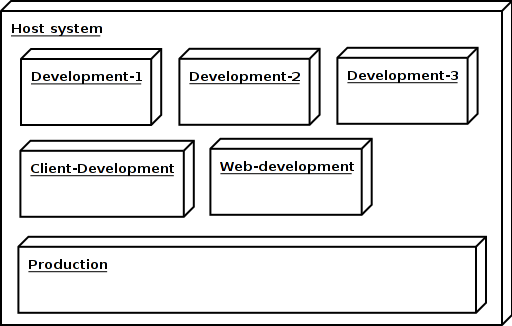
\includegraphics{Vagrant-illustration.png}
\caption{Illustration of system setup}
\end{figure}

The system is entirely scripted, that is, everything can be set up using
the scripts located in the vagrant git\footnote{git.cs.umu.se, access required.}. The
scripts located under \texttt{scripts/provision} deal with the virtual
environments, while the scripts under \texttt{scripts/environment} deal
with the server, such as setting up the firewall and external
directories used by the virtual machines.

\subsection{Using the toolchain}\label{sec:using-the-toolchain}

This is a short introduction to the tools used in the environments.

\subsubsection{Using gnu screen}\label{sec:using-gnu-screen}

To ensure processes run even when nobody has a terminal open to the
server \texttt{screen} is used. \texttt{screen} is a terminal
multiplexer, which could be viewed as a in-terminal window manager. To
start a new screen you run the command

\begin{verbatim}
$ screen
\end{verbatim}

which then starts a \texttt{screen} and attaches your current terminal
to it. \texttt{screen} is controlled by prefixing a command with a
modifier. For example, to detach from a \texttt{screen} window, you use
\texttt{\textless{}C-a\textgreater{}} which you then release, indicating
you wish to send a command to \texttt{screen}. You then press
\texttt{d}, which is the hot-key for \emph{detach}. You are now detached
from the screen.

You might not be surprised when I tell you that several \texttt{screen}
windows can be running at the same time. To list the currently running
\texttt{screen} sessions, you run the command

\begin{verbatim}
$ screen -list
\end{verbatim}

If there is only one session running, you can attach to it using simply
the command

\begin{verbatim}
$ screen -r
\end{verbatim}

to attach. If there are several running \texttt{screens}, you must
specify which session to attach to. The following is an example of this.
It starts two sessions, \texttt{first} and \texttt{second} in a detached
state. The \texttt{-dmS} flag means they are started in a detached
state. We then list the sessions and see that several are running, as
expected.

\begin{verbatim}
[vagrant@localhost ~]$ screen -dmS "first"
[vagrant@localhost ~]$ screen -dmS "second"
[vagrant@localhost ~]$ screen -list
There are screens on:
    15073.second    (Detached)
    15053.first (Detached)
2 Sockets in /var/run/screen/S-vagrant.
\end{verbatim}

We can now attach to these sessions by running the command, replacing
\texttt{\textless{}session-name} with the name of your session.

\begin{verbatim}
$ screen -S <session name>
\end{verbatim}

To terminate a \texttt{screen}, attach to it and run \texttt{exit}.

\subsection{Configured environments}\label{sec:configured-environments}

The environments as currently configured are described below.

\subsubsection{Production}\label{sec:production}

This environment runs the production code. Hands off if you are unsure
of or have not communicated your change clearly to everyone else.

\begin{itemize}
\itemsep1pt\parskip0pt\parsep0pt
\item
  Virtual hardware

  \begin{itemize}
  \itemsep1pt\parskip0pt\parsep0pt
  \item
    45000 MB RAM
  \item
    8 CPU Cores
  \end{itemize}
\item
  Ports

  \begin{itemize}
  \itemsep1pt\parskip0pt\parsep0pt
  \item
    Genomizer-server: 7000
  \item
    Http: 80
  \item
    Https: 443
  \end{itemize}
\item
  Local IP: 192.168.33.10
\item
  Directories

  \begin{itemize}
  \itemsep1pt\parskip0pt\parsep0pt
  \item
    Temporary files

    \begin{itemize}
    \itemsep1pt\parskip0pt\parsep0pt
    \item
      External directory: \texttt{/Data/tmp}
    \item
      Internal directory: \texttt{/tmp}
    \end{itemize}
  \item
    Data files

    \begin{itemize}
    \itemsep1pt\parskip0pt\parsep0pt
    \item
      External directory: \texttt{/Data/production-data}
    \item
      Internal directory: \texttt{/data}
    \end{itemize}
  \end{itemize}
\end{itemize}

\subsubsection{Development-1}\label{sec:development-1}

This environment is assigned to the \texttt{database} group.

\begin{itemize}
\itemsep1pt\parskip0pt\parsep0pt
\item
  Virtual hardware

  \begin{itemize}
  \itemsep1pt\parskip0pt\parsep0pt
  \item
    4000 MB RAM
  \item
    1 CPU Core
  \end{itemize}
\item
  Ports

  \begin{itemize}
  \itemsep1pt\parskip0pt\parsep0pt
  \item
    Genomizer-server: 7001
  \item
    Http: 8081
  \item
    Https: 4431
  \end{itemize}
\item
  Local IP: 192.168.33.11
\item
  Directories

  \begin{itemize}
  \itemsep1pt\parskip0pt\parsep0pt
  \item
    Temporary files

    \begin{itemize}
    \itemsep1pt\parskip0pt\parsep0pt
    \item
      External directory: \texttt{/Data/development-1-tmp}
    \item
      Internal directory: \texttt{/tmp}
    \end{itemize}
  \item
    Data files

    \begin{itemize}
    \itemsep1pt\parskip0pt\parsep0pt
    \item
      External directory: \texttt{/Data/development-1-data}
    \item
      Internal directory: \texttt{/data}
    \end{itemize}
  \end{itemize}
\end{itemize}

\subsubsection{Development-2}\label{sec:development-2}

This environment is assigned to the \texttt{business-logic} group.

\begin{itemize}
\itemsep1pt\parskip0pt\parsep0pt
\item
  Virtual hardware

  \begin{itemize}
  \itemsep1pt\parskip0pt\parsep0pt
  \item
    4000 MB RAM
  \item
    1 CPU Core
  \end{itemize}
\item
  Ports

  \begin{itemize}
  \itemsep1pt\parskip0pt\parsep0pt
  \item
    Genomizer-server: 7002
  \item
    Http: 8082
  \item
    Https: 4432
  \end{itemize}
\item
  Local IP: 192.168.33.12
\item
  Directories

  \begin{itemize}
  \itemsep1pt\parskip0pt\parsep0pt
  \item
    Temporary files

    \begin{itemize}
    \itemsep1pt\parskip0pt\parsep0pt
    \item
      External directory: \texttt{/Data/development-2-tmp}
    \item
      Internal directory: \texttt{/tmp}
    \end{itemize}
  \item
    Data files

    \begin{itemize}
    \itemsep1pt\parskip0pt\parsep0pt
    \item
      External directory: \texttt{/Data/development-2-data}
    \item
      Internal directory: \texttt{/data}
    \end{itemize}
  \end{itemize}
\end{itemize}

\subsubsection{Development-3}\label{sec:development-3}

This environment is assigned to the \texttt{processing} group.

\begin{itemize}
\itemsep1pt\parskip0pt\parsep0pt
\item
  Virtual hardware

  \begin{itemize}
  \itemsep1pt\parskip0pt\parsep0pt
  \item
    4000 MB RAM
  \item
    1 CPU Core
  \end{itemize}
\item
  Ports

  \begin{itemize}
  \itemsep1pt\parskip0pt\parsep0pt
  \item
    Genomizer-server: 7003
  \item
    Http: 8083
  \item
    Https: 4433
  \end{itemize}
\item
  Local IP: 192.168.33.13
\item
  Directories

  \begin{itemize}
  \itemsep1pt\parskip0pt\parsep0pt
  \item
    Temporary files

    \begin{itemize}
    \itemsep1pt\parskip0pt\parsep0pt
    \item
      External directory: \texttt{/Data/development-3-tmp}
    \item
      Internal directory: \texttt{/tmp}
    \end{itemize}
  \item
    Data files

    \begin{itemize}
    \itemsep1pt\parskip0pt\parsep0pt
    \item
      External directory: \texttt{/Data/development-3-data}
    \item
      Internal directory: \texttt{/data}
    \end{itemize}
  \end{itemize}
\end{itemize}

\subsubsection{Client-development}\label{sec:client-development}

This environment is assigned to the \texttt{desktop} group.

\begin{itemize}
\itemsep1pt\parskip0pt\parsep0pt
\item
  Virtual hardware

  \begin{itemize}
  \itemsep1pt\parskip0pt\parsep0pt
  \item
    4000 MB RAM
  \item
    1 CPU Core
  \end{itemize}
\item
  Ports

  \begin{itemize}
  \itemsep1pt\parskip0pt\parsep0pt
  \item
    Genomizer-server: 7004
  \item
    Http: 8084
  \item
    Https: 4434
  \end{itemize}
\item
  Local IP: 192.168.33.14
\item
  Directories

  \begin{itemize}
  \itemsep1pt\parskip0pt\parsep0pt
  \item
    Temporary files

    \begin{itemize}
    \itemsep1pt\parskip0pt\parsep0pt
    \item
      External directory: \texttt{/Data/development-client-tmp}
    \item
      Internal directory: \texttt{/tmp}
    \end{itemize}
  \item
    Data files

    \begin{itemize}
    \itemsep1pt\parskip0pt\parsep0pt
    \item
      External directory: \texttt{/Data/development-client-data}
    \item
      Internal directory: \texttt{/data}
    \end{itemize}
  \end{itemize}
\end{itemize}

\subsubsection{Web-development}\label{sec:web-development}

This environment is assigned to the \texttt{web} and \texttt{app}
groups.

\begin{itemize}
\itemsep1pt\parskip0pt\parsep0pt
\item
  Virtual hardware

  \begin{itemize}
  \itemsep1pt\parskip0pt\parsep0pt
  \item
    4000 MB RAM
  \item
    1 CPU Core
  \end{itemize}
\item
  Ports

  \begin{itemize}
  \itemsep1pt\parskip0pt\parsep0pt
  \item
    Genomizer-server: 7005
  \item
    Http: 8085
  \item
    Https: 4435
  \end{itemize}
\item
  Local IP: 192.168.33.15
\item
  Directories

  \begin{itemize}
  \itemsep1pt\parskip0pt\parsep0pt
  \item
    Temporary files

    \begin{itemize}
    \itemsep1pt\parskip0pt\parsep0pt
    \item
      External directory: \texttt{/Data/development-web-tmp}
    \item
      Internal directory: \texttt{/tmp}
    \end{itemize}
  \item
    Data files

    \begin{itemize}
    \itemsep1pt\parskip0pt\parsep0pt
    \item
      External directory: \texttt{/Data/development-web-data}
    \item
      Internal directory: \texttt{/data}
    \end{itemize}
  \end{itemize}
\end{itemize}

\subsection{The important scripts}\label{sec:the-important-scripts}

The machines are configured using a myriad of scripts with various
responsibilities. The \texttt{Vagrantfile} defines how the virtual
machine is built. This includes which provisioning files are to be
executed, and how much memory and resources to give the machine. It also
configures the port forwarding into the machine, and which shared data
folders are available to the machine. Messing with these configurations
is inadvisable.

The \texttt{Vagrantfile} runs, as previously said, configuration
scripts. Their names and basic responsibilities are listed below. Unless
otherwise specified, they are located under \texttt{scripts/provision}.

\begin{enumerate}
\itemsep1pt\parskip0pt\parsep0pt
\item
  \texttt{install\_apache.sh} - Installs and configures the apache
  server. It installs the config files \texttt{httpd.conf},
  \texttt{ssl.conf}, and \texttt{proxy.conf} located under
  \texttt{scripts/provision/config}, along with running the
  \texttt{install\_certificates} script.
\item
  \texttt{install\_postgresql.sh} - While the name may seem confusing,
  this installs \texttt{puppet} and the \texttt{puppet/postgresql}
  module. This allows the \texttt{Vagrantfile} to run puppet
  provisioning on the machine to install postgresql with the settings
  provided in \texttt{manifests/build.pp}.
\item
  \texttt{install\_certificates.sh} - This is an expect script, which is
  run by the \texttt{install\_apache} script. This is introduced to deal
  with the fact that you need to respond to questions to generate a SSL
  certificate. It generates a SSL certificate, and moves it to the
  correct location.
\item
  \texttt{install\_utils.sh} - There are some tools and utilities which
  were requested or needed by the scripts or persons working on the
  project. They are installed from this script.
\item
  \texttt{install\_startup\_scripts.sh} - Installs various scripts that
  are used for server administration.
\item
  \texttt{install\_genomizer\_server.sh} - Installs the genomizer-server
\item
  \texttt{install\_genomizer\_webclient.sh} - Installs the genomizer-web
  client to the apache server.
\end{enumerate}

If you are confused by what a script does, reading it can give you a
clearer picture of what it does.

\subsection{Creating a new
environment}\label{sec:creating-a-new-environment}

\subsubsection{Considerations}\label{sec:considerations}

Before setting up a new environment, you should consider the memory and
CPU footprint inherent in running a virtual machine. The host machine as
currently configured can run 6 environments with no noticeable slowdown,
with five machines at 1 cpu core and 4GB of RAM, and a production
environment that is assigned 8 CPU cores and 45GB of RAM. It is not
recommended to exceed this configuration, as unexpected side-effects
could occur.

\subsubsection{Checking out the correct
files}\label{sec:checking-out-the-correct-files}

When building a new environment, you may wish to configure which
versions of the server software and web client software the script
installs. By default, the scripts are configured to fetch the
\texttt{master} branch of the \texttt{genomizer-server} and the
\texttt{master} branch of the \texttt{genomizer-web} application. These
settings are modified by editing the
\texttt{scripts/provision/install\_genomizer\_server.sh} and
\texttt{scripts/provision/install\_genomizer\_webclient.sh}
respectively.

In order to change the version of the \texttt{genomizer-server}, edit
the \texttt{scripts/
provision/install\_genomizer\_server.sh} script.
Locate the line(s)


\begin{Shaded}
\begin{Highlighting}[numbers=left,,]
\CommentTok{# We checkout the master version by default}
\KeywordTok{git} \NormalTok{checkout master}
\end{Highlighting}
\end{Shaded}

and replace them with


\begin{Shaded}
\begin{Highlighting}[numbers=left,,]
\CommentTok{# We checkout the <desired branch> version by default}
\KeywordTok{git} \NormalTok{checkout }\KeywordTok{<}\NormalTok{desired branch}\KeywordTok{>}
\end{Highlighting}
\end{Shaded}

To change the version of the \texttt{genomizer-web} client, edit the
\texttt{scripts/provision/} \texttt{install\_genomizer\_webclient.sh}
script. Locate the line(s)


\begin{Shaded}
\begin{Highlighting}[numbers=left,,]
\CommentTok{# We run the master branch by default}
\KeywordTok{cd} \NormalTok{genomizer-web}
\KeywordTok{git} \NormalTok{checkout master}
\end{Highlighting}
\end{Shaded}

and replace them with


\begin{Shaded}
\begin{Highlighting}[numbers=left,,]
\CommentTok{# We run the <desired branch> branch by default}
\KeywordTok{cd} \NormalTok{genomizer-web}
\KeywordTok{git} \NormalTok{checkout }\KeywordTok{<}\NormalTok{desired branch}\KeywordTok{>}
\end{Highlighting}
\end{Shaded}

\subsubsection{Setting up the files}\label{setting-up-the-files}

When setting up the new environment, you may (or may not) want to run it
with the same settings as the production environment. In this section
all relevant settings are explained and motivated.

\paragraph{Editing the Vagrantfile}\label{editing-the-vagrantfile}

In the vagrant file, the primarily interesting settings are concerning
\emph{port forwarding}, \emph{local ip}, \emph{synced folders}, and
\emph{memory}. Given that you wish to customize the environment, the
\emph{provision} settings might be of use as well. The
\texttt{Vagrantfile} is written in a Ruby DSL.

The port forwarding settings looks as follows.

\hyperdef{}{portforwarding}{\label{portforwarding}}
\begin{Shaded}
\begin{Highlighting}[numbers=left,,]
\NormalTok{config.vm.network }\StringTok{"forwarded_port"}\NormalTok{, guest: }\DecValTok{80}\NormalTok{, host:}\DecValTok{8080}
\NormalTok{config.vm.network }\StringTok{"forwarded_port"}\NormalTok{, guest: }\DecValTok{7000}\NormalTok{, host:}\DecValTok{7000}
\NormalTok{config.vm.network }\StringTok{"forwarded_port"}\NormalTok{, guest: }\DecValTok{443}\NormalTok{, host:}\DecValTok{4443}
\end{Highlighting}
\end{Shaded}

The \texttt{host} field defines which port the virtual machine binds on
in the host machine, while the \texttt{guest} defines the port the
virtual machine it binds on internally.

To define which \textbf{local IP} the virtual machine runs on, you
modify the line below to suit your needs. Note that the IP must be
unique, and it is recommended to stay inside the \texttt{192.168.33.x}
subnet.

\hyperdef{}{privatenetwork}{\label{privatenetwork}}
\begin{Shaded}
\begin{Highlighting}[numbers=left,,]
\NormalTok{config.vm.network }\StringTok{"private_network"}\NormalTok{, ip: }\StringTok{"192.168.33.10"}
\end{Highlighting}
\end{Shaded}

You may also need to mount a folder from the host machine as a drive
inside the virtual machine. This is achieved by editing or adding to the
lines shown below. The first argument is the hosts path to the folder to
share, and the second is where the virtual machine should mount it.

\hyperdef{}{syncedfolder}{\label{syncedfolder}}
\begin{Shaded}
\begin{Highlighting}[numbers=left,,]
\NormalTok{config.vm.synced_folder }\StringTok{"/Data/production-data"}\NormalTok{, }\StringTok{"/data"}
\NormalTok{config.vm.synced_folder }\StringTok{"/Data/production-tmp"}\NormalTok{, }\StringTok{"/tmp"}
\end{Highlighting}
\end{Shaded}

The actual hardware specifications given to the virtual machine is
defined by these lines:


\begin{Shaded}
\begin{Highlighting}[numbers=left,,]
\NormalTok{config.vm.provider }\StringTok{"virtualbox"} \KeywordTok{do} \NormalTok{|vb|}
    \NormalTok{vb.memory = }\StringTok{"45000"}
    \NormalTok{vb.cpus = }\DecValTok{8}
\KeywordTok{end}
\end{Highlighting}
\end{Shaded}

These lines define that the machine should run with 45000 MB of RAM, and
run on 8 CPU cores. If other settings are desired, you modify these
lines. For example, the development environments might look like


\begin{Shaded}
\begin{Highlighting}[numbers=left,,]
\NormalTok{config.vm.provider }\StringTok{"virtualbox"} \KeywordTok{do} \NormalTok{|vb|}
    \NormalTok{vb.memory = }\StringTok{"4000"}
    \NormalTok{vb.cpus = }\DecValTok{1}
\KeywordTok{end}
\end{Highlighting}
\end{Shaded}

\paragraph{Editing the settings.cfg}\label{editing-the-settings.cfg}

The \texttt{settings.cfg} file contains the settings that are installed
to the genomizer-server. These should need no modification, except
perhaps to edit the tunneling settings.

If you however do want to edit some settings, note that the database
settings must correspond to the ones configured in \texttt{build.pp},
else the server will fail to connect to the database.

The settings available in the server settings are straightforward, and
are commented such that no further explanation is required.

\paragraph{Editing the httpd.conf}\label{editing-the-httpd.conf}

The \texttt{httpd.conf} file is dead-standard, except for the very last
few lines. These lines assures that SSL is forced, and that any traffic
connecting to the non-SSL apache is told to reconnect with SSL.

\hyperdef{}{code}{\label{code}}
\begin{Shaded}
\begin{Highlighting}[]
\KeywordTok{<VirtualHost} \ErrorTok{*:80}\KeywordTok{>}
    \NormalTok{RedirectPermanent / https://130.239.192.110}
\KeywordTok{</VirtualHost>}
\end{Highlighting}
\end{Shaded}

You may wish to edit where this reroutes to as needed.

\paragraph{Modifying the build.pp}\label{modifying-the-build.pp}

The \texttt{build.pp} file details how the postgresql database is
constructed, along with which sql files are automatically run on the
server. It is not recommended to change how this file functions except
to change the password and modify which sql files are run.

\paragraph{\texorpdfstring{Creating the \texttt{tmp} and \texttt{data}
folders}{Creating the tmp and data folders}}\label{creating-the-tmp-and-data-folders}

When constructing an environment, the machine requires a place to store
temporary files, and a place to store large data files. These are by
default placed in
\texttt{/Data/\textless{}environment\textgreater{}-tmp} and
\texttt{/Data/\textless{}environment\textgreater{}-data}. To create
these folders, and give them the correct permissions, you should run the
following commands. The \texttt{\textless{}your-user\textgreater{}}
should be replaced with the user that runs the virtual machines, and
\texttt{\textless{}environment\textgreater{}} with the name of your
environment.

\begin{verbatim}
[user@your-environment]$ sudo mkdir /Data/<environment>-tmp
[user@your-environment]$ sudo mkdir /Data/<environment>-data
[user@your-environment]$ sudo chown -R <your-user> /data/<environment>-tmp
[user@your-environment]$ sudo chmod -R 1777 /data/<environment>-tmp
[user@your-environment]$ sudo chmod -R 777 /data/<environment>-data
\end{verbatim}

\subsubsection{Running the new
environment}\label{running-the-new-environment}

Once you have created an environment, you need to allow vagrant to
construct the associated virtual machine. This is done by running
\texttt{vagrant\ up} in the directory associated with your environment.

Vagrant should now start building the virtual machine, along with
provisioning it. It will write a lot of information to the terminal you
run it in, and this is perfectly normal. The build takes on average 5-10
minutes to complete.

Once it has finished, the environment is up and running, except for one
detail: \texttt{genomizer-server} is not running. You can start it by
typing the following into the terminal.

\begin{verbatim}
[user@environment]$ vagrant ssh
Last login: Tue May 12 12:4032 2015 from 10.0.2.2
[vagrant@localhost]$ bash startup.sh
\end{verbatim}

If you wish to view the server process, this can be done by running

\begin{verbatim}
[vagrant@localhost]$ screen -r
\end{verbatim}

which attaches to the screen created by \texttt{startup.sh}.

\subsection{Modifying an existing
environment}\label{modifying-an-existing-environment}

While it is very useful to build an environment from scratch, you do not
always want to do everything from scratch. You want to \emph{modify} an
existing environment. Modifying an environment is fairly straight
forward, you simply edit the configuration files, as shown in
\emph{Creating a new environment}. Once you have modified the files
according to your preferences, you run

\begin{verbatim}
[user@your-environment]$ vagrant destroy && vagrant up
\end{verbatim}

if you wish to \emph{completely} rebuild the machine. If you simply want
the machine to reload the \texttt{Vagrantfile} settings, you can run

\begin{verbatim}
[user@your-environment]$ vagrant reload
\end{verbatim}

\paragraph{Checkout new branches}\label{checkout-new-branches}

If you decide that you wish to run another branch in the environment,
and do not wish to rebuild the environment, you can simply ssh into the
vagrant machine and checkout using git as you normally would, compiling
and running as you would normally.

\begin{verbatim}
[user@your-environment]$ vagrant ssh
[vagrant@localhost]$ cd genomizer-server
[vagrant@localhost]$ git stash
[vagrant@localhost]$ git checkout <branch>
[vagrant@localhost]$ git stash pop
[vagrant@localhost]$ ant clean build jar
[vagrant@localhost]$ java -jar server.jar
\end{verbatim}

In this context, the \texttt{stash} ensures that our modified
\texttt{settings.cfg} is preserved. If for some reason
\texttt{settings.cfg} is overwritten, you can get a fresh copy from
\texttt{/vagrant/scripts/provision/config/settings.cfg} inside the
virtual machine.

\subsection{Rebuilding an environment}\label{rebuilding-an-environment}

Rebuilding an environment is dead simple, simply run

\begin{verbatim}
[user@your-environment]$ vagrant destroy && vagrant up
\end{verbatim}

\subsection{Deleting an environment}\label{deleting-an-environment}

\textbf{NOTE: The changes explained in this chapter are irreversible!}

To delete an environment it is not sufficient to simply remove the
folder containing the environment. The virtual machine must also be
deleted. The following steps removes an environment cleanly.

\begin{enumerate}
\itemsep1pt\parskip0pt\parsep0pt
\item
  Enter the environment folder.
\item
  Destroy the virtual machine with \texttt{vagrant\ destroy}.
\item
  Remove the \texttt{.vagrant} folder.
\item
  Remove the environment folder.
\item
  Remove the environments \texttt{tmp} and \texttt{data} folders.
\end{enumerate}

The \texttt{tmp} and \texttt{data} folders are by default located under
\texttt{/Data/\textless{}environment\textgreater{}-tmp} and
\texttt{/Data/\textless{}environment\textgreater{}-data}.

\subsection{Configuring the host
system}\label{configuring-the-host-system}

Please note, all of these things can be achieved by running the script
\texttt{scripts/
environment/setup\_host\_environment.sh}, provided a
CentOS host system. \textbf{Never run this script without reading it
through. Seriously.} Even if you want to configure manually, reading
this script is useful to get examples of the commands that are relevant.

\subsubsection{External folders and their
permissions.}\label{external-folders-and-their-permissions.}

The host machine is required to make available storage space for the
virtual machines. By default this is assumed to be \texttt{/Data}. In
this folder, you should place \texttt{tmp} and \texttt{data} folders --
one for each environment -- with the permissions 1777 for \texttt{tmp}.
The \texttt{data} folder should have the permissions 777. The
\texttt{tmp} folder must be owned by the vagrant user.

\subsubsection{Configuring the firewall}\label{configuring-the-firewall}

The firewall needs to allow \emph{at least} the ports \texttt{80},
\texttt{443} and \texttt{7000}. There is a script which configures these
settings under \texttt{scripts/environment/iptables\_config.sh}. The
only advanced setting here is a workaround to patch reserved ports into
the virtual machines without requiring root permissions.

The firewall is instructed to reroute traffic to port \texttt{80} to the
port \texttt{8080} and traffic to the port \texttt{443} to the port
\texttt{4443} which then the virtual machine can bind on.

\begin{figure}[htbp]
\centering
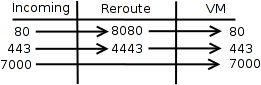
\includegraphics[width=0.6\textwidth]{routing1.png}
\caption{Illustration of rerouting}
\end{figure}

Specifics on how to run these commands are illustrated in
\texttt{iptables\_config.sh}.

\subsubsection{Prerequisite software}\label{prerequisite-software}

The setup requires \texttt{vagrant} and \texttt{virtualbox} to be
installed.

\paragraph{Virtualbox}\label{virtualbox}

To install virtualbox, you can run the following commands. Replace
\texttt{\$VAGRANT\_USER} with the vagrant user.

\hyperdef{}{installvirtualbox}{\label{installvirtualbox}}
\begin{Shaded}
\begin{Highlighting}[numbers=left,,]
\CommentTok{# Get the EPEL repo}
\KeywordTok{rpm} \NormalTok{-Uvh https://download.fedoraproject.org/pub/epel/7/x86_64/e/\textbackslash{}}
    \NormalTok{epel-release-7-5.noarch.rpm}

\CommentTok{# Install kernel headers and devel tools}
\KeywordTok{yum} \NormalTok{-y install kernel-devel kernel-headers dkms}
\KeywordTok{yum} \NormalTok{groupinstall }\StringTok{"Development Tools"}
\KeywordTok{yum} \NormalTok{update}

\CommentTok{# Install oracle public key}
\KeywordTok{wget} \NormalTok{http://download.virtualbox.org/virtualbox/debian/\textbackslash{}}
    \NormalTok{oracle_vbox.asc}
\KeywordTok{rpm} \NormalTok{--import oracle_vbox.asc}
\KeywordTok{rm} \NormalTok{-rf oracle_vbox.asc}

\CommentTok{# Add the virtualbox repo}
\KeywordTok{wget} \NormalTok{http://download.virtualbox.org/virtualbox/rpm/el/\textbackslash{}}
    \NormalTok{virtualbox.repo -O /etc/yum.repos.d/virtualbox.repo}
\KeywordTok{yum} \NormalTok{update }\CommentTok{# Update repo info for safety}

\CommentTok{# Time to actually install virtualbox}
\KeywordTok{yum} \NormalTok{-y install VirtualBox-4.3}
\KeywordTok{service} \NormalTok{vboxdrv setup }\CommentTok{# Setup vbox driver}
\KeywordTok{usermod} \NormalTok{-a -G vboxusers }\OtherTok{$VAGRANT_USER} \CommentTok{# Add VB user}
\end{Highlighting}
\end{Shaded}

\paragraph{Vagrant}\label{vagrant}

To install vagrant, you can run the following commands.

\hyperdef{}{installvagrant}{\label{installvagrant}}
\begin{Shaded}
\begin{Highlighting}[numbers=left,,]
\KeywordTok{wget} \NormalTok{https://dl.bintray.com/mitchellh/vagrant/\textbackslash{}}
    \NormalTok{vagrant_1.7.2_x86_64.rpm}
\KeywordTok{rpm} \NormalTok{-ivh vagrant_1.7.2_x86_64.rpm}
\KeywordTok{rm} \NormalTok{-rf vagrant_1.7.2_x86_64.rpm}
\end{Highlighting}
\end{Shaded}



